
\section{Matrix power} 
\label{sec:matrix-power}
In this section, we define the matrix power, which can be seen as a way of representing several trees in one. %Roughly speaking, the several trees are the contents of registers in a register automaton.
%, and the single tree that represents them is the computation tree of the register automaton.  We then show that several trees stored in a computation  can be unfolded in a derivable way. 

\begin{definition}
    [Matrix power] For $k \in \set{1,2,\ldots}$ define the $k$-th matrix power\footnote{
        The name  matrix power is based the matrix power in  universal algebra (for the latter, see~\cite{Taylor1975} or~\cite{szendrei1990simple}). Roughly speaking, the restrictions that we place on the original definition correspond to the single-use and monotone conditions from Definition~\ref{def:stt}. 
     } of a ranked set $\rSigma$ 
to be 
\begin{align*}
 \mati k \rSigma \quad \eqdef \quad \ranked{\reduce k \rSigma^k}.
\end{align*}
\end{definition}

Here is a picture of a binary element in the matrix power, where $k=3$:
\begin{center}
\includegraphics[scale=.4, page=85]{pics.pdf}
\end{center}

A matrix power of arity $n$ is used as an abstraction of an $n$-ary register update $\ranked{R\to \tmonad(\Gamma+R+\dots+R)}$. The number $k$ represents the number of registers (that is the size of $\ranked {R}$), and each letter from $\rSigma$ represents a register update (that is, an element of $\ranked{\tmonad(\Gamma+R+\dots+R)}$). When two letters share the same port in the matrix power, this means that the corresponding register updates call the same component of $\ranked{R+\dots+R}$ in their definition, the position in the fold indicates which precise register is called. For instance, the register update above is an abstraction of the following binary register update of registers $r, s$ and $t$:
   \begin{center}
   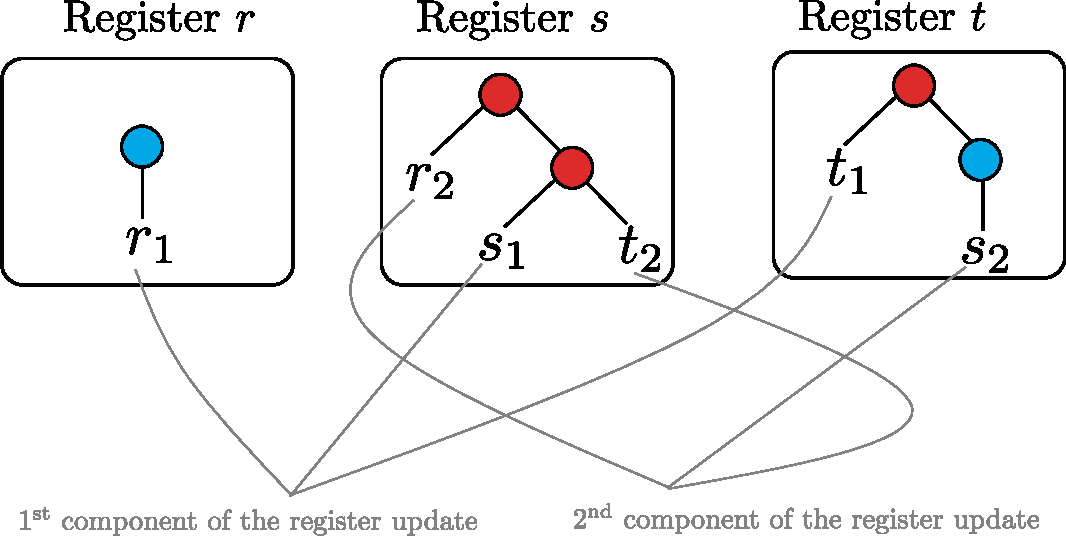
\includegraphics[scale=.34]{register-update-matrix-power.pdf}
   \end{center}
When we run a STT on an input tree, we decorate it with register updates following the transition function. In order to evaluate this tree, the first thing to do is to determine, for each register update of the root, its "dependency tree" that is to say the register updates they call, inductively. When register updates are abstracted by matrix powers, this operation of determining the dependency tree is what we call \emph{unfolding}. We illustrate it by the following example 
\begin{center}
\includegraphics[scale=.28, page=39]{pics.pdf}
\end{center}
Formally, \emph{unfolding} is a function of type
\begin{align*}
    \ranked{\unfold : \tmonad \mati k \rSigma \to \mati k {(\tmonad \Sigma)} }
    \end{align*}
 which is defined as follows by induction on the size of the input term. If the input is an empty term, then the output is this term:
\begin{center}
\includegraphics[scale=.3, page=83]{pics.pdf}
\end{center}
Otherwise, if the input is a nonempty term $a(t_1,\ldots,t_n)$ then the output is obtained by first applying unfolding to to the smaller terms $t_1,\ldots,t_n$, and then applying the following derivable function, which we call \emph{shallow unfold}. 
\begin{align*}
    \ranked{
        \xymatrix{
            \shallowterm{\mati k \rSigma} {\mati k \rGamma}  \ar[r] & \mati k {(\shallowterm \Sigma \Gamma)}.
        }
    }
\end{align*}
Here is a picture of unfolding for shallow terms:
\begin{center}
\includegraphics[scale=.2, page=86]{pics.pdf}
\end{center}
More formally, unfolding for shallow terms is defined to be   the composition of the following functions
    \begin{align*}
        \xymatrix@C=3.2cm{
          {\begin{array}{c}
          \shallowterm{\mati k \rSigma} {\mati k \rGamma} \\{=\shallowterm{\reduce k {\Sigma^k}}{\reduce k {\Gamma^k}}}
          \end{array}}  \ar[d]_{{\mathrm{Commutativity}}}\ar[r]^{\mathrm{Shallow\  unfold}} &  {\begin{array}{c}
         \ranked{\mati k {(\shallowterm \Sigma \Gamma)}} \\=  \ranked{ \reduce k(\shallowterm{\Sigma}{ {\Gamma}})^k}
          \end{array}} \\
             \reduce k(\shallowterm{\reduce k {\Sigma^k}}{ {\Gamma^k}})  \ar[r]_{{\mathrm{Matching}}} &  \ranked{ \reduce k(\shallowterm{\Sigma^k}{ {\Gamma}}) } \ar[u]_{\mathrm{Commutativity}} 
        } 
    \end{align*}
Since our atomic functions and combinators do not have any general mechanisms for induction, it is not clear how to derive the unfolding operation. In fact, it is not derivable in general, but it will become derivable after imposing a monotonicity requirement.   To see the need for monotonicity, consider the following example.
\begin{example}\label{eq:twist}
    Consider the following elements in a second matrix power:
\begin{center}
\includegraphics[scale=.3, page=84]{pics.pdf}
\end{center}
Let $t_n \in \trees \mati 2 \rSigma$ be the tree which consists of a path with $n$ nodes using the unary label $a$, followed by a leaf with label $b$. If we apply term unfolding to this tree, and then project to the first coordinate, then we get a tree with a white leaf if and only if  $n$ is even.  If term unfolding were derivable, then thanks to the results from Section~\ref{sec:to-transductions}  we would get a first-order tree-to-tree transduction 
\begin{align*}
\trees \redset{a,b} \to \trees \rSigma
\end{align*}
where the output would contain a white leaf if and only if the input has odd depth. This is in turn would imply that having even depth for trees over $\redset{a,b}$ is first-order definable, which it is not, because first-order logic cannot do modulo counting.
\end{example}

The problem in the above example is that the letter $a$ does a swap on its ports, which leads to counting modulo two. To forbid such swaps, we impose a monotonicity requirement that matches the monotonicity requirement for register updates in register transducers.
For a port $i$ in an element of the matrix power $a/f \in \mati k \rSigma$ define its \emph{twist} to be the partial function from $\set{1,\ldots,k}$ to itself 
which is the composition of 
\begin{align*}
\xymatrix{
    \set{1,\ldots,k} \ar[r]^-{j \mapsto {(j,i)}} & \set{1,\ldots,k} \times \set{1,\ldots,n} \ar[r]^-{f^{-1}} & \set{1,\ldots,\arity a} \ar[r] & \set{1,\ldots,k}
},
\end{align*}
where the last function maps each port of the tuple $a$ to the coordinate of the tuple that created that port. Here is a picture:
\begin{center}
\includegraphics[scale=.3, page=87]{pics.pdf}
\end{center}
 We say that an element of the $k$-matrix power is \emph{monotone} if all of its ports have monotone twist.
 We are now ready to state the principal result of this section.

\begin{proposition}\label{prop:monotone-unfold}
    For every finite ranked set $\rSigma$ and every $k \in \set{1,2,\ldots}$ there is a derivable function 
    \begin{align*}
    \ranked{ f : \tmonad \mati k \Sigma \to \mati k {(\tmonad \Sigma)}}
    \end{align*}
    which coincides with term unfolding for monotone inputs.
\end{proposition}
The proof of the  above lemma is one of the main technical contributions of this paper, and it is given in the appendix. One of the ingredients of the proof is a first-order (in fact, derivable) version of the Factorisation Forest Theorem for trees, which is based in Colcombet's splits from~\cite{colcombetCombinatorialTheoremTrees2007}.  

\begin{corollary}\label{cor:matrix-power}
    Let $\rSigma$ be a finite set and let $\rDelta \subseteq \mati k \rSigma$ be a finite set which contains only monotone elements. Then one can derive the tree-to-tree function
    \begin{align*}
    f : \trees \rDelta \to \trees \rSigma  \qquad t \mapsto \text{first tree in the unfolding of $t$.}
    \end{align*}
\end{corollary}
% Let $\alg$ be an algebra and let $k \in \set{1,2,\ldots}$. How should the $k$-th power of the algebra be defined? For the domain, we use  $k$-tuples from the domain of $\alg$.  What about the operations? A natural   approach is to define the $n$-ary operations to be  $k$-tuples of $n$-ary operations from $\alg$, acting coordinate-wise. Because of the coordinate-wise action,  the coordinates in the product are independent of each other. This will be insufficient for our intended application, where the algebra $\alg$ is meant to represent individual register automaton, since the contents of register $r$ in the output of a register update depend on the contents of other registers in the input valuation . To  model this interdependence, we use a more sophisticated notion of power, 
% defined below.
% \begin{definition}
%     For an algebra $\alg$ and $k \in \set{1,2,\ldots}$, the $k$-th matrix power\footnote{
%         The definition of matrix power that we use is a special case of the original definition of matrix power from universal algebra (for the latter, see~\cite{Taylor1975} or~\cite{szendrei1990simple}). Roughly speaking, the restrictions that we place on the original definition correspond to the single-use and monotone conditions from Definition~\ref{def:stt}. 
%     } of $\alg$ is defined as follows. The domain and signature are defined by
%     \begin{align*}
%     \overbrace{(\algdom \alg)^k}^{\text{domain}} \qquad \overbrace{
%         \ranked{\reduce k ((\algops \alg)^k)}}^{\text{signature}}
%         \end{align*}
%         while the  shallow product operation is defined by
%         \begin{align*}
%             \ranked{
%         \xymatrix{
%             \shallowterm {\reduce k (\algops \alg)^{k}} {{(\algdom \alg)}^k} \ar[d] \\
%             \shallowterm {(\algops \alg)^{k}} {{(\algdom \alg)}} \ar[d] \\
%             (\shallowterm {(\algops \alg)} {{(\algdom \alg)}})^k
%          \ar[d]\\
%             (\algdom \alg)^k
%         }
%         }
%         \end{align*}
% \end{definition}

% By definition, if an algebra has a derivable shallow product, then the same is true for its  matrix powers, i.e.~for every $k$ the shallow product in the $k$-th matrix power is derivable. The following proposition -- which is much harder to show -- states a similar implication for  (not necessarily shallow) products.  
% \begin{proposition}\label{prop:matrix-power} If an algebra has a derivable product, then the same is true for its matrix powers.
% \end{proposition}
%


